
% --- CAPÍTULO 4 ---
\chapter{Desenvolvimento}
Esta seção detalha o processo de desenvolvimento do modelo de predição de diabetes, abordando a arquitetura do projeto, o fluxo de execução do pipeline, a funcionalidade de cada módulo de código, as tecnologias e bibliotecas empregadas, e os resultados obtidos. O objetivo é fornecer uma compreensão aprofundada da implementação técnica e das decisões tomadas para construir uma solução robusta e eficaz na identificação precoce de casos de diabetes tipo 2.

\section{Dados}
O conjunto de dados selecionado para este estudo foi o Diabetes Prediction Dataset, disponibilizado na plataforma Kaggle por Iammustafa\cite{Iammustafa2022}. O dataset é composto por registros de pacientes, com diversas variáveis clínicas e demográficas que visam prever a presença ou ausência de diabetes, ele é composto por 100.000 registros, cada um representando um indivíduo com diversas características clínicas e comportamentais, e uma variável alvo indicando a presença ou ausência de diabetes.

O conjunto de dados apresenta características clínicas que serão detalhadas na Tabela 1. 

% Tabela 1
\begin{table}[H]
    \centering
    \caption{Descrição das Características usadas no conjunto de dados.}
    \label{tab:features}
    \begin{tabular}{@{}ll@{}}
        \toprule
        \textbf{Característica} & \textbf{Descrição} \\
        \midrule
        gender & gênero \\
        age & idade \\
        hypertension & hipertensão \\
        heart disease & doença cardíaca \\
        smoking history & histórico de tabagismo \\
        bmi & Índice de Massa Corporal \\
        HbA1c level & nível de Hemoglobina Glicada \\
        blood glucose level & nível de glicose no sangue \\
        diabetes & "variável alvo: 0 para não diabético, 1 para diabético" \\
        \bottomrule
    \end{tabular}
\end{table}

É relevante destacar que o dataset reflete uma distribuição de classes significativa, onde a maioria das instâncias corresponde a indivíduos sem diabetes. A variável alvo diabetes apresenta um desbalanceamento, com 8\% dos pacientes diagnosticados com diabetes e 92\% sem o diagnóstico essa distribuição é demonstrada na figura 10. Essa característica do dataset é crucial para o processo de modelagem, exigindo a aplicação de técnicas específicas para mitigar o viés em favor da classe majoritária, como o SMOTE, que será detalhado na seção 4.1.1.

\begin{figure}[H]
    \centering
    \caption{Distribuição da variável alvo diabetes no Diabetes Prediction Dataset.}
    \label{fig:dist}
    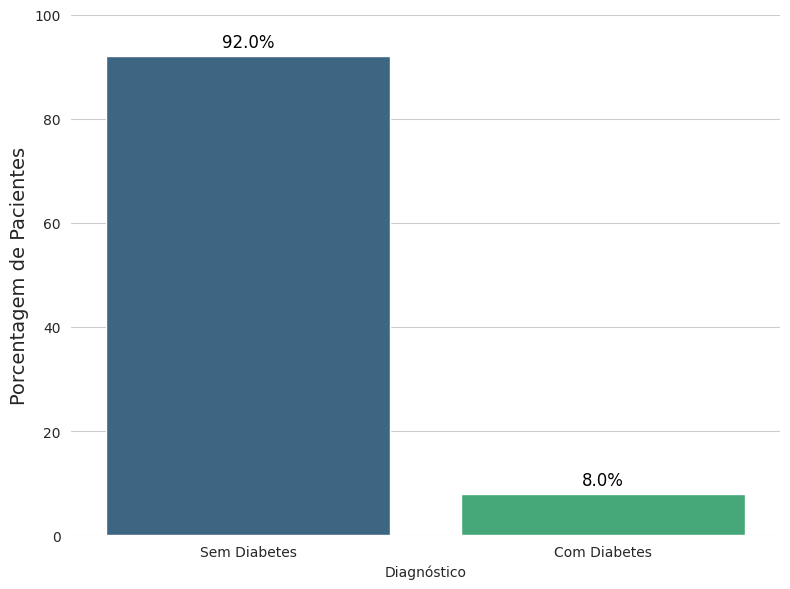
\includegraphics[width=0.8\textwidth]{figuras/distribuicao.png} 
    \par 
     \small Fonte: Elaborado pelo autor
\end{figure}


A qualidade e a abrangência das informações contidas neste dataset o tornam um recurso valioso para a aplicação de técnicas de aprendizado de máquina na predição de doenças, oferecendo um cenário realista para o desenvolvimento e validação de modelos preditivos em saúde.

\subsection{Normalização dos Dados}
A normalização dos dados foi uma etapa essencial do pré-processamento e utilizou a padronização por Z-score, que transforma cada atributo para média 0 e desvio padrão 1. No pipeline, essa padronização é aplicada após o tratamento de outliers numéricos via limites de IQR, garantindo que todas as features entrem no modelo na mesma escala. 

A técnica SMOTE também foi aplicada para mitigar o desbalanceamento de classes no conjunto de treino. Ela cria amostras sintéticas da classe minoritária, após tratamento de outliers, codificação one-hot e padronização por Z-score, evitando vazamento de informação, os conjuntos de validação e teste não foram reajustados. Esta estratégia aumentou a representatividade da classe minoritária como podemos ver na figura 11, e reduziu o viés de previsão e melhorou métricas como recall e AUC-ROC, sem comprometer a avaliação do modelo.

\begin{figure}[H]
    \centering
    \caption{Distribuição ajustada com SMOTE.}
    \label{fig:smite}
    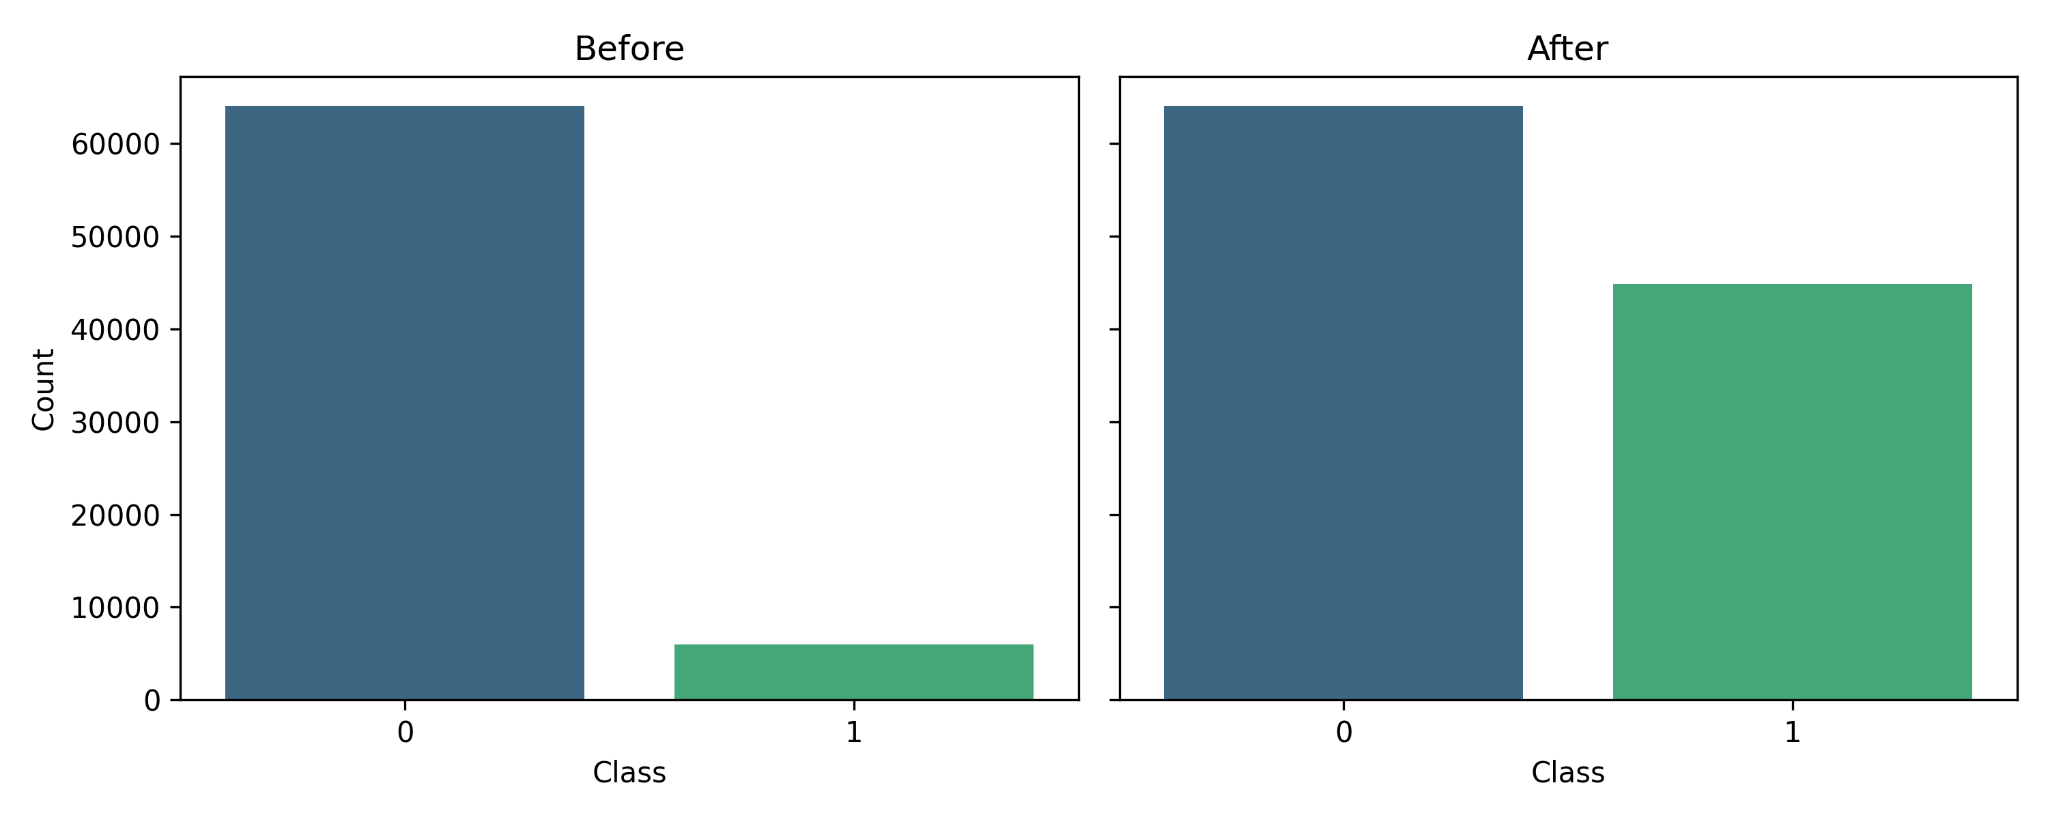
\includegraphics[width=1\textwidth]{figuras/distribuicao smote.png} 
    \par 
     \small Fonte: Elaborado pelo autor
\end{figure}

A normalização de dados é fundamental para otimizar o desempenho do modelo, pois padroniza a escala dos recursos. Essa padronização melhora a interpretabilidade, acelera a convergência e previne problemas de gradiente causados por magnitudes desiguais. Além disso, a normalização favorece a comparabilidade e a interpretabilidade de coeficientes e importâncias de atributos, uma vez que coloca os atributos na mesma unidade, contribuindo para um desempenho mais robusto dos modelos.

\subsection{Divisão dos Dados De Treinamento e Teste}
Para o treinamento, o conjunto de dados foi dividido, dimensionado e transformado em subconjuntos de treinamento e teste, utilizando a função train\_test\_split da biblioteca scikit-learn.

Do conjunto de dados original, 20\% foram reservados para testes. O restante foi então dividido de forma estratificada, com 70\% para treino e 10\% para validação. A utilização de uma semente aleatória fixa garantiu a reprodutibilidade dos resultados. Essa metodologia permite uma avaliação imparcial com dados nunca antes vistos e a calibração precisa dos modelos através do conjunto de validação. 


\section{Métricas De Detecção de Qualidade}
A avaliação do desempenho de um modelo de Machine Learning é um passo crítico para garantir sua eficácia e confiabilidade, especialmente em tarefas de classificação como a predição de diabetes. As métricas de detecção de qualidade fornecem uma quantificação do quão bem o modelo está realizando suas previsões, permitindo a comparação entre diferentes abordagens e a identificação de áreas para melhoria. A escolha das métricas apropriadas depende do problema em questão e das características do conjunto de dados, como o balanceamento das classes \cite{Han2012, Bishop2006}.

Para modelos de classificação, as métricas são frequentemente derivadas da Matriz de Confusão, que detalha os resultados das previsões em relação aos valores reais. As principais métricas incluem Acurácia, Precisão, Recall e F1-Score, cada uma oferecendo uma perspectiva diferente sobre o desempenho do modelo \cite{Freitas2024}. Para problemas de regressão, como a predição de um valor contínuo, métricas como o RMSE são mais adequadas. A seguir, serão detalhadas as métricas relevantes para a avaliação do modelo de predição de diabetes.

\subsection{Matriz De Confusão}
A Matriz de Confusão é uma tabela que sumariza o desempenho de um algoritmo de classificação, apresentando a contagem de previsões corretas e incorretas feitas pelo modelo em comparação com os valores reais. Ela é particularmente útil para entender os tipos de erros que o modelo está cometendo, especialmente em problemas de classificação binária \cite{Strauss2022}.

A matriz é composta por quatro elementos principais:

\begin{figure}[H]
    \centering
    \caption{Matriz de confusão.}
    \label{fig:cf}
    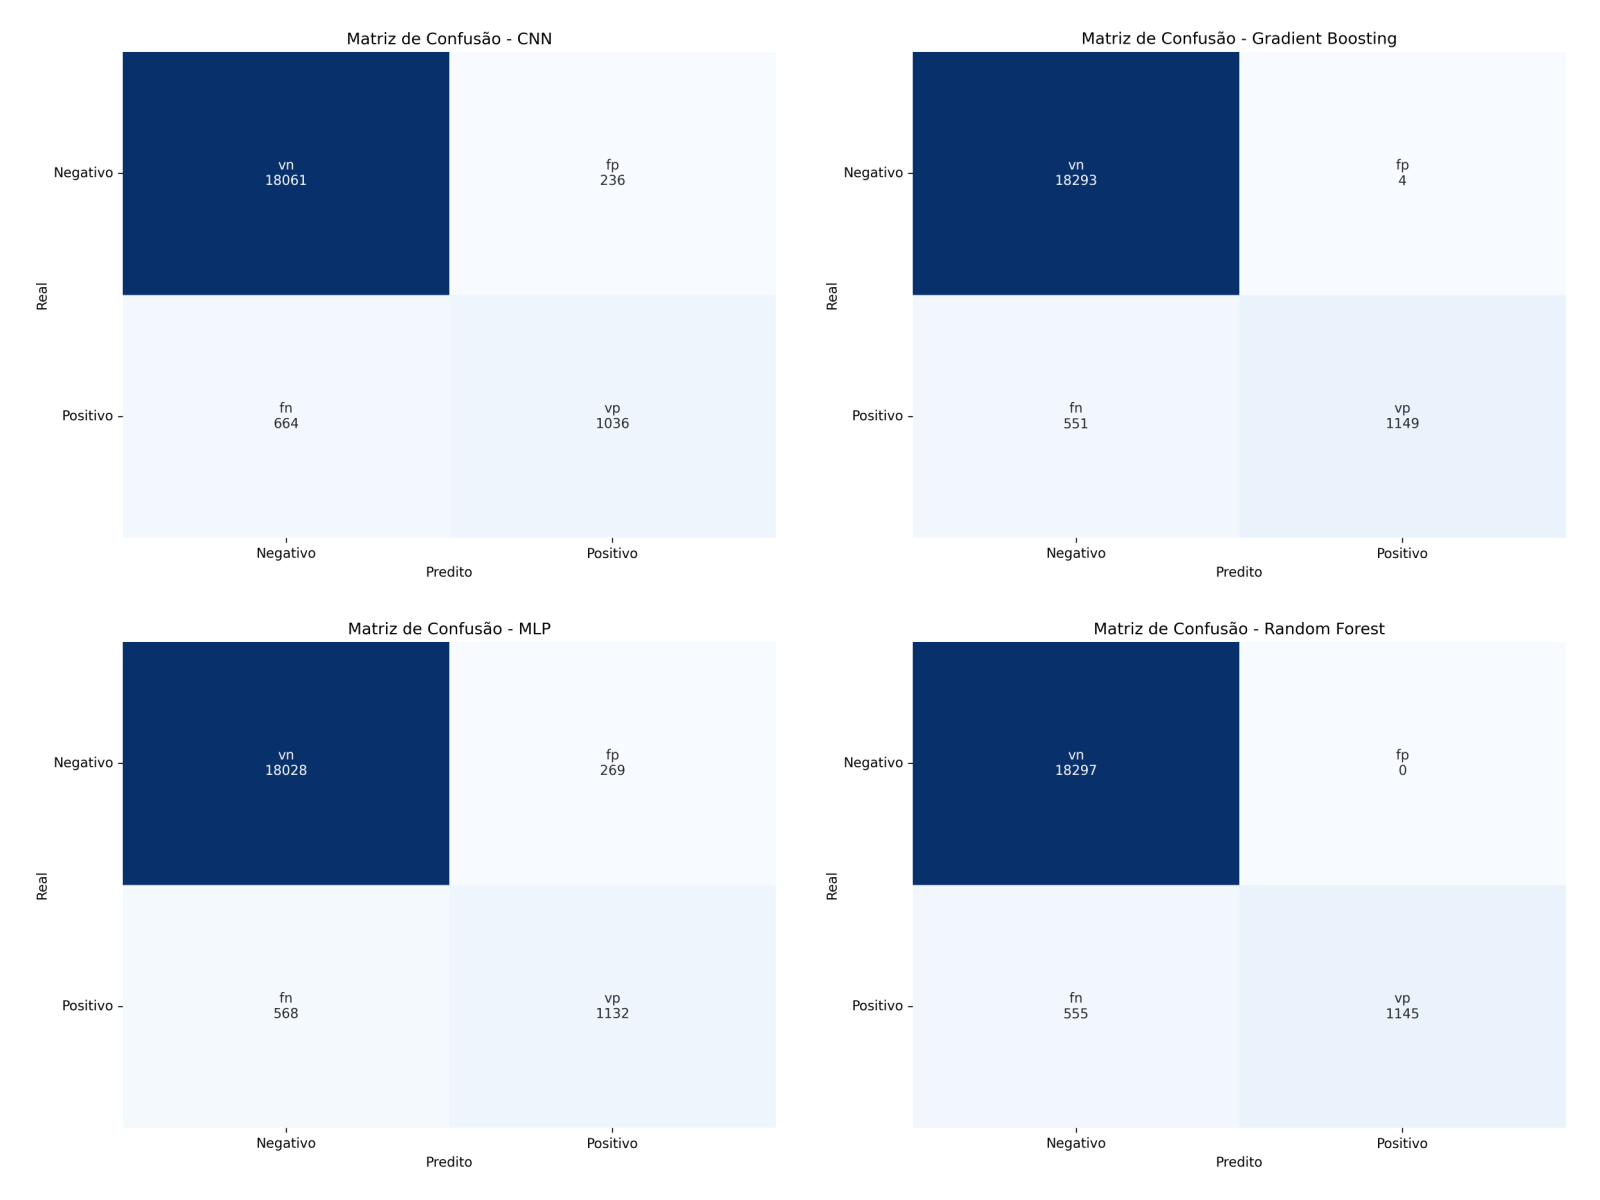
\includegraphics[width=0.8\textwidth]{figuras/matriz confusao exemplo.png} 
    \par 
    \small Fonte: Elaborado pelo autor.)
\end{figure}

\begin{itemize}
    \item \textbf{Verdadeiro Positivo (VP):} O modelo previu corretamente a classe positiva (ex: previu que o indivíduo tem diabetes e ele realmente tem).
    \item \textbf{Verdadeiro Negativo (VN):} O modelo previu corretamente a classe negativa (ex: previu que o indivíduo não tem diabetes e ele realmente não tem).
    \item \textbf{Falso Positivo (FP):} O modelo previu incorretamente a classe positiva por exemplo previu que o indivíduo tem diabetes, mas ele não tem.
    \item \textbf{Falso Negativo (FN):} O modelo previu incorretamente a classe negativa como por exemplo, previu que o indivíduo não tem diabetes, mas ele tem. 
\end{itemize}

A estrutura da Matriz de Confusão é a seguinte:

\begin{center}
\begin{tabular}{|l|l|l|}
\hline
 & \textbf{Previsto Positivo} & \textbf{Previsto Negativo} \\
\hline
\textbf{Real Positivo} & Verdadeiro Positivo (VP) & Falso Negativo (FN) \\
\hline
\textbf{Real Negativo} & Falso Positivo (FP) & Verdadeiro Negativo (VN) \\
\hline
\end{tabular}
\end{center}

Através da Matriz de Confusão, é possível calcular diversas métricas de desempenho que fornecem uma visão mais aprofundada sobre a qualidade do modelo, indo além da simples acurácia \cite{Pighini2025}.

\subsection{Acurácia}
A Acurácia é a métrica mais intuitiva e amplamente utilizada para avaliar o desempenho de um modelo de classificação. Ela representa a proporção de previsões corretas em relação ao total de previsões realizadas. Em outras palavras, a acurácia mede a porcentagem de vezes que o modelo fez a previsão correta.
A fórmula para calcular a Acurácia é:
$$ \text{Accuracy} = \frac{\text{correct classifications}}{\text{total classifications}} = \frac{VP + VN}{VP+VN+FP+FN} $$
Onde:
\begin{itemize}
    \item VP = Verdadeiro Positivo
    \item VN = Verdadeiro Negativo
    \item FN = Falso Negativo
    \item FP = Falso Positivo
\end{itemize}
Embora a acurácia seja fácil de entender e calcular, ela pode ser enganosa em cenários onde as classes são desbalanceadas. Por isso, é crucial analisar a acurácia em conjunto com outras métricas, especialmente em problemas de saúde onde a detecção de casos positivos é de extrema importância \cite{Hastie2009}.

\subsection{Loss}
A função de perda, ou loss function, é um componente fundamental no treinamento de modelos de Machine Learning. Ela quantifica a diferença entre as previsões do modelo e os valores reais dos dados. O objetivo do treinamento de um modelo é minimizar essa função de perda, ajustando os pesos e vieses da rede para que suas previsões se tornem cada vez mais próximas dos valores reais \cite{Goodfellow2016}.

A escolha da função de perda depende do tipo de problema que está sendo resolvido:

Para tarefas de classificação, funções de perda comuns incluem:
\begin{itemize}
    \item \textbf{Binary Cross-Entropy (Entropia Cruzada Binária):} Utilizada para problemas de classification binária, onde há apenas duas classes possíveis.
    \item \textbf{Categorical Cross-Entropy (Entropia Cruzada Categórica):} Usada para problemas de classificação multiclasse, onde há mais de duas classes.
\end{itemize}

Para tarefas de regressão, funções de perda comuns incluem:
\begin{itemize}
    \item \textbf{Mean Squared Error (MSE - Erro Quadrático Médio):} Calcula a média dos quadrados das diferenças entre os valores previstos e os valores reais.
    \item \textbf{Mean Absolute Error (MAE - Erro Absoluto Médio):} Calcula a média dos valores absolutos das diferenças entre os valores previstos e os valores reais.
\end{itemize}
Durante o treinamento, o algoritmo de otimização utiliza o valor da função de perda para determinar a direção e a magnitude dos ajustes nos parâmetros do modelo. Uma função de perda bem escolhida é crucial para guiar o modelo a aprender padrões significativos nos dados e a generalizar bem para dados não vistos.

\subsection{Precisão}
A Precisão é uma métrica que avalia a qualidade das previsões positivas do modelo. Uma alta precisão indica que o modelo tem poucos Falsos Positivos, ou seja, ele raramente classifica incorretamente uma instância negativa como positiva \cite{Freitas2024}.
A fórmula para calcular a Precisão é:
$$ \text{Precision} = \frac{\text{correctly classified actual positives}}{\text{everything classified as positive}} = \frac{VP}{VP+FP} $$
Onde:
\begin{itemize}
    \item VP = Verdadeiro Positivo
    \item FP = Falso Positivo
\end{itemize}
Em um contexto de predição de diabetes, uma alta precisão é importante para minimizar o número de falsos alarmes, evitando que indivíduos saudáveis sejam erroneamente diagnosticados com a doença, o que poderia gerar ansiedade desnecessária e custos com exames adicionais. No entanto, um modelo com alta precisão pode ter um baixo Recall, ou seja, pode deixar de identificar muitos casos reais de diabetes.

\subsection{Recall}
O Recall é uma métrica que avalia a capacidade do modelo de identificar todas as instâncias positivas reais. Ela responde à pergunta: “Das instâncias que realmente são positivas, quantas o modelo conseguiu identificar corretamente?” . Um alto Recall indica que o modelo tem poucos Falsos Negativos, ou seja, ele raramente deixa de identificar uma instância positiva \cite{Freitas2024}.
A fórmula para calcular o Recall é:
$$ \text{Recall} = \frac{\text{correctly classified actual positives}}{\text{all actual positives}} = \frac{VP}{VP+FN} $$
Onde:
\begin{itemize}
    \item VP = Verdadeiro Positivo
    \item FN = Falso Negativo
\end{itemize}
Em um contexto de predição de diabetes, um alto Recall é crucial para garantir que a maioria dos indivíduos com a doença seja identificada, minimizando o risco de falsos negativos. Deixar de identificar um caso real de diabetes pode ter consequências graves para a saúde do paciente, pois o tratamento precoce é essencial. No entanto, um modelo com alto Recall pode ter uma baixa precisão, ou seja, pode gerar muitos falsos positivos.

\subsection{F1 Score}
O F1 Score é uma métrica que combina a Precisão e o Recall em uma única pontuação, sendo a média harmônica dessas duas métricas. Ele é particularmente útil quando há um desequilíbrio entre as classes no conjunto de dados (ou seja, uma classe é muito mais frequente que a outra) e quando Falsos Positivos e Falsos Negativos têm custos semelhantes. O F1 Score busca um equilíbrio entre Precisão e Recall, penalizando modelos que performam bem em uma métrica, mas mal na outra \cite(Han2012).
A fórmula para calcular o F1 Score é:
$$ \text{F1 Score} = \frac{VP}{VP + \frac{VP+FN}{2}} $$
Onde:
\begin{itemize}
    \item VP = Verdadeiro Positivo
    \item FN = Falso Negativo
\end{itemize}
Um F1 Score alto indica que o modelo tem tanto alta precisão quanto alto recall. Em problemas de saúde, onde tanto a identificação correta de pacientes doentes quanto a minimização de diagnósticos errados são importantes, o F1 Score pode ser uma métrica mais representativa do desempenho geral do modelo do que a acurácia isoladamente.


\section{Construção Dos Modelos}
A arquitetura central adotada neste estudo é a Multi-Layer Perceptron (MLP), cuja escolha é justificada por sua comprovada eficácia e ampla utilização como baseline robusto para problemas de classificação com dados tabulares \cite{Goodfellow2016}. O MLP é intrinsecamente adequado para modelar relações não-lineares complexas, considerando o conjunto de features de forma global e totalmente conectadas.

Adicionalmente, com o objetivo estritamente comparativo, uma arquitetura de Rede Neural Convolucional (CNN) foi implementada. Embora a CNN seja uma abordagem para domínios como visão computacional, sua aplicação em dados tabulares não é trivial, mas serve here como um contraponto metodológico. A inclusão da CNN visa contrastar o desempenho do modelo padrão com uma arquitetura de paradigma distinto, que opera através da extração de padrões locais. Esta comparação permite avaliar se o modelo MLP padrão é de fato suficiente para o problema ou se uma topologia não convencional, mesmo que não seja teoricamente a primeira escolha, pode oferecer resultados competitivos. A busca por hiperparâmetros foi empregada para otimizar e avaliar imparcialmente ambas as topologias, visando a seleção de um modelo eficaz.

\subsection{Otimização Bayesiana Aplicada Seleção de Hiperparâmetros}
Para a definição dos modelos de redes neurais, optou-se por um processo automatizado de ajuste de hiperparâmetros por meio da otimização bayesiana. Este método foi escolhido por sua eficiência superior quando comparado a abordagens como a busca aleatória.

A seleção de hiperparâmetros adequados representa um dos maiores desafios no desenvolvimento de redes neurais, uma vez que o espaço de busca cresce exponencialmente com o número de parâmetros configuráveis. Para este trabalho, implementou-se uma estratégia de otimização bayesiana que explora inteligentemente um vasto espaço de configurações possíveis para as redes neurais aplicadas à predição de diabetes.

A otimização bayesiana resolve esse problema através de uma abordagem probabilística que modela a relação entre hiperparâmetros e desempenho do modelo usando processos gaussianos. Diferentemente de métodos tradicionais como busca aleatória ou busca em grade, que tratam cada experimento de forma independente, o otimizador bayesiano aprende com os resultados anteriores para decidir quais configurações testar a seguir. O algoritmo mantém uma distribuição de probabilidade sobre o espaço de hiperparâmetros e utiliza uma função de aquisição para balancear exploitation e exploration.

A implementação utiliza o Keras Tuner com parâmetros específicos ajustados para o problema: 5 pontos iniciais exploratórios são gerados aleatoriamente para estabelecer uma base de conhecimento inicial, seguidos por seleção bayesiana guiada para os trials subsequentes. Os parâmetros alpha e beta da função de aquisição foram configurados para favorecer uma exploração moderada do espaço, evitando convergência prematura para ótimos locais. Cada configuração testada é avaliada com múltiplas execuções para considerar a variabilidade estocástica do treinamento de redes neurais.

Durante o processo de busca, o algoritmo executa cada trial por um número predefinido de épocas, coletando métricas de desempenho incluindo precisão, acurácia, AUC-ROC, recall e perda tanto para os conjuntos de treino quanto de validação. Um mecanismo de early stopping monitora a métrica objetivo e interrompe o treinamento caso não haja melhoria por 20 épocas consecutivas, economizando tempo computacional sem comprometer a qualidade da avaliação. Esta estratégia permite que configurações promissoras treinem até convergência enquanto configurações ruins são descartadas rapidamente.

A cada trial concluído, o otimizador bayesiano atualiza seu modelo probabilístico do espaço de hiperparâmetros, refinando sua compreensão sobre quais regiões são mais promissoras. Esta abordagem adaptativa permite que o algoritmo concentre seus recursos computacionais nas áreas do espaço de busca com maior probabilidade de conter a configuração ótima. Na prática, isso significa que enquanto uma busca aleatória de 50 trials poderia desperdiçar recursos testando configurações claramente subótimas, a otimização bayesiana direciona progressivamente seus testes para configurações cada vez mais refinadas.

Ao final da otimização, o sistema gera automaticamente estatísticas comparativas, as cinco melhores configurações e salva o modelo de melhor desempenho com seus hiperparâmetros em JSON, garantindo reprodutibilidade. A análise temporal registra o tempo médio por trial e o tempo total de execução.

A otimização Bayesiana supera a busca aleatória, atingindo configurações de alta performance mais rapidamente e com menos experimentos. Sua eficiência é crucial para o ajuste de hiperparâmetros em redes neurais, especialmente com recursos computacionais e tempo limitados.

\subsubsection{Os Modelos Escolhidos}
A otimização de hiperparâmetros revelou uma disparidade de desempenho substancial entre as arquiteturas propostas. O modelo MLP selecionado configurou-se como uma rede profunda de 5 camadas ocultas, caracterizada por uma arquitetura complexa, um misto de funções de ativação e uso intensivo de técnicas de regularização, como Batch Normalization em quatro camadas, altos níveis de Dropout e regularização L2. Utilizando o Nadam otimizador, este modelo atingiu 71.03\% de precisão na validação e um recall de 80,82\%.

Em contrapartida, o modelo CNN, incluído para fins comparativos, emergiu como a arquitetura superior, alcançando 86,93\% de precisão na validação. A arquitetura vencedora é um modelo híbrido 1D-CNN composto por uma base convolucional de 3 camadas atuando como extratora de features, seguida por uma cabeça de classificação (MLP) densa de 2 camadas. Este modelo também utilizou forte regularização, mas aplicou Batch Normalization apenas nas camadas densas. Notavelmente, o melhor desempenho foi obtido com o otimizador SGD, uma escolha mais simples que o Nadam utilizado pelo MLP.

\subsection{Avaliação dos modelos}
Para uma análise de desempenho comparativa e aprofundada, indo além da métrica de acurácia, foram geradas Matrizes de Confusão para todos os modelos avaliados: MLP, CNN, RandomForestClassifier e GradientBoostingClassifier. Estas matrizes, apresentadas na figura 12, são cruciais no contexto do diagnóstico de diabetes, pois permitem avaliar os tipos de erros específicos que cada arquitetura comete.

\begin{figure}[H]
    \centering
    \caption{Matriz de Confusão.}
    \label{fig:cm}
    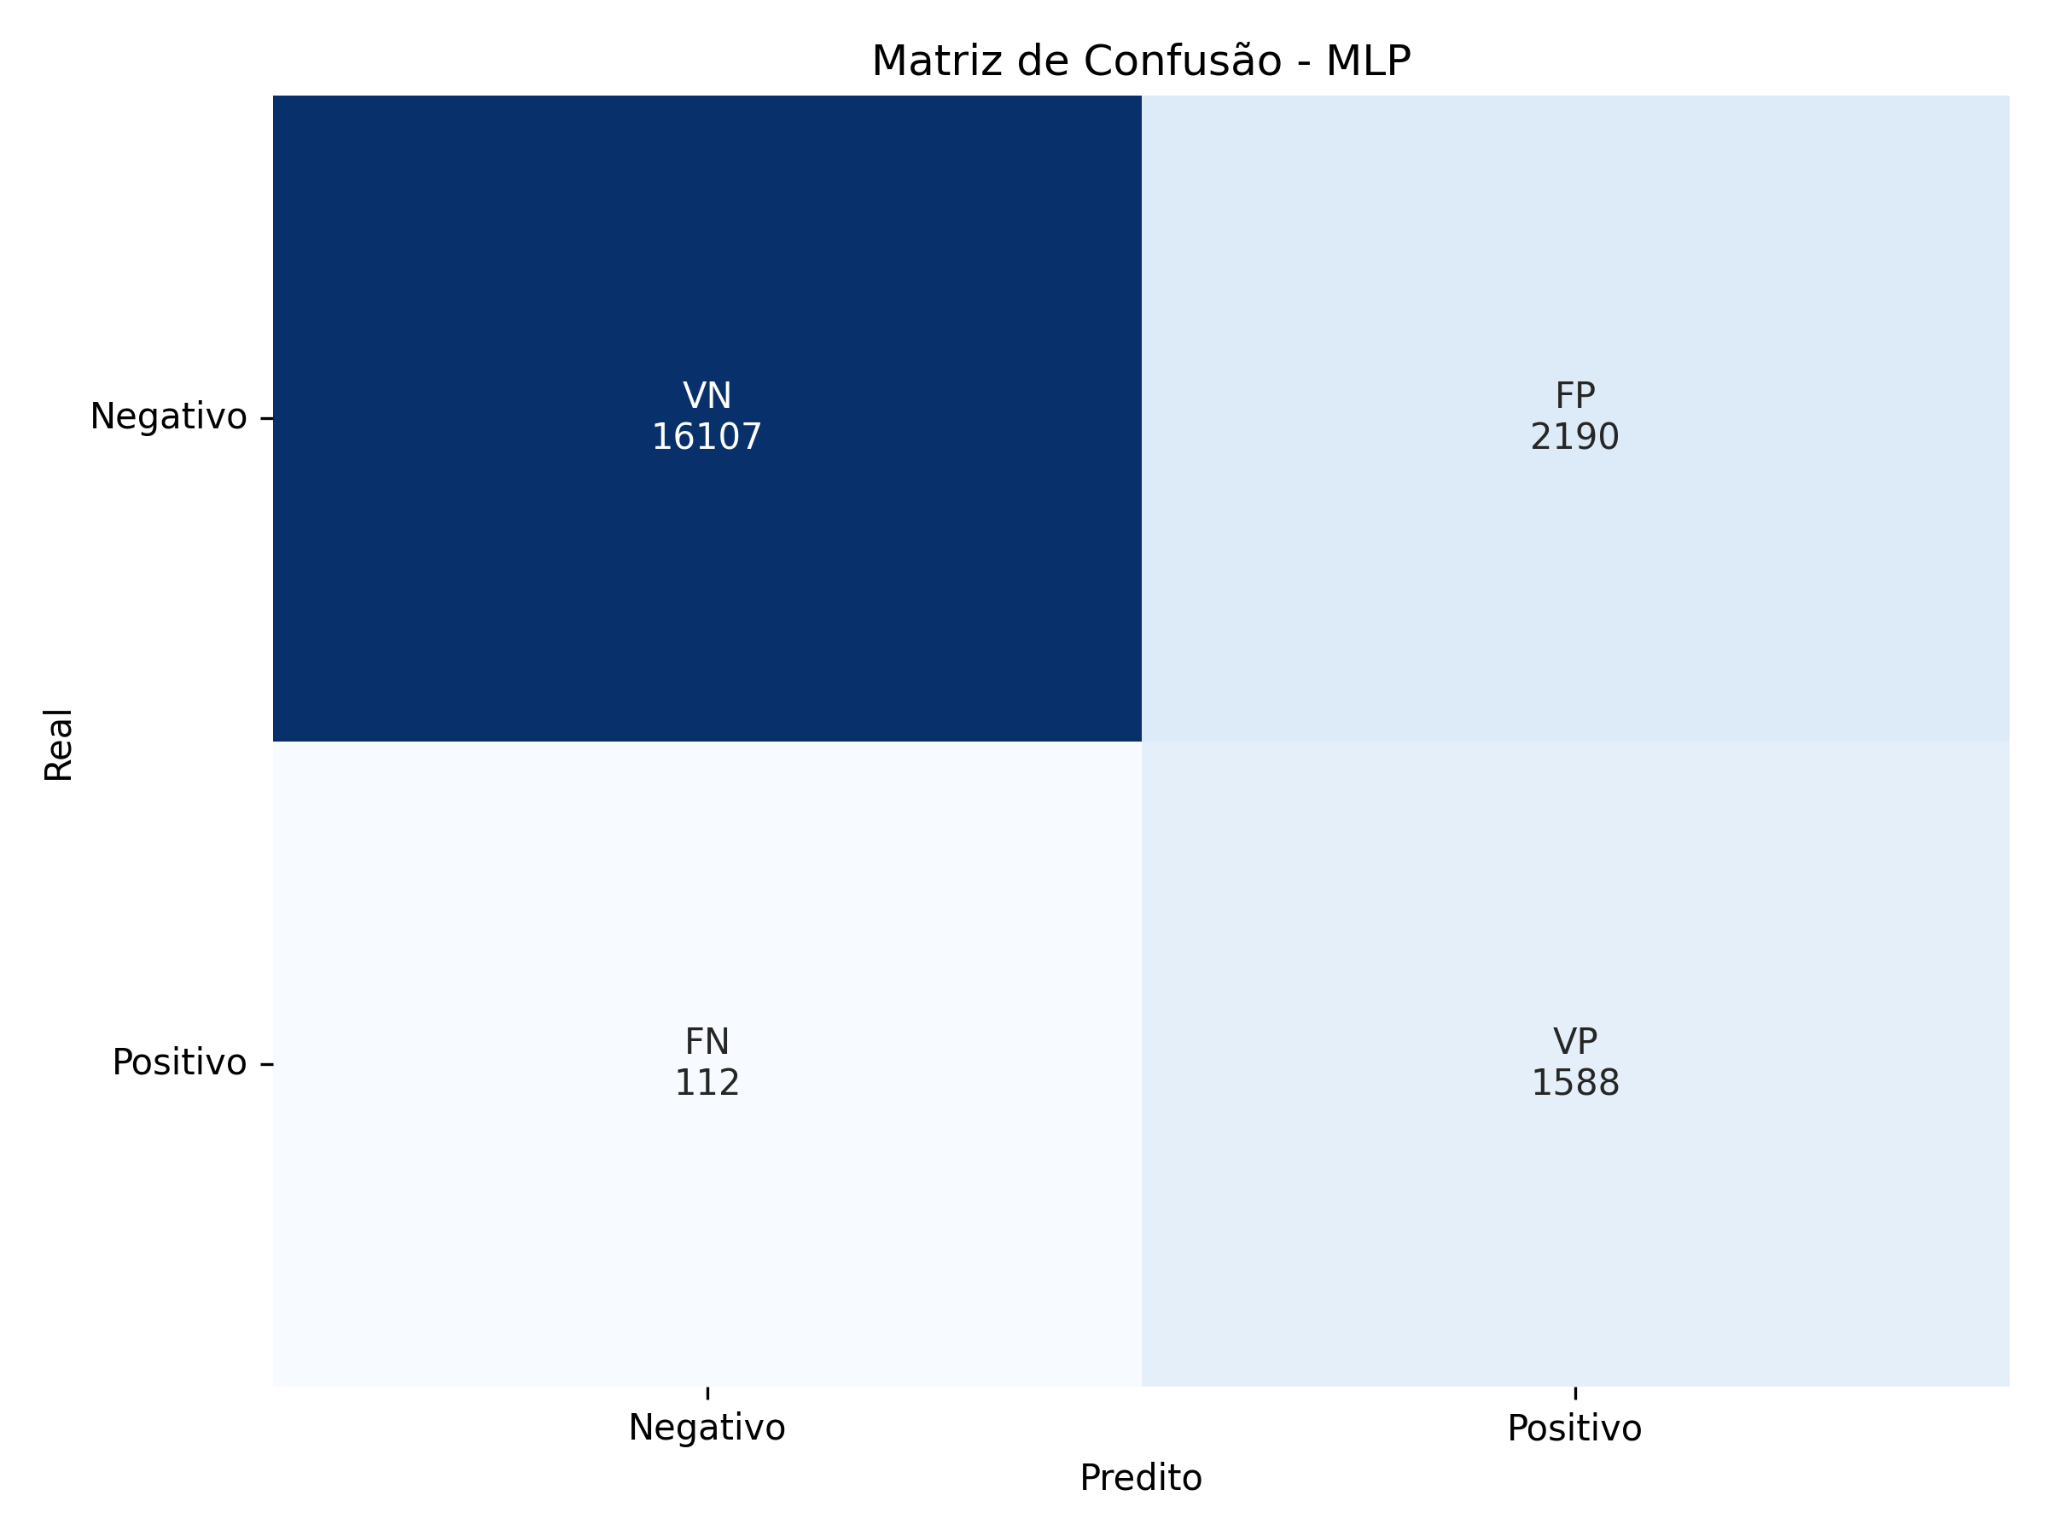
\includegraphics[width=0.8\textwidth]{figuras/cf.png} 
    \par 
     \small Fonte: Elaborado pelo autor
\end{figure}

Na predição desta doença, existem dois erros principais a considerar: o Falso Positivo, que ocorre quando o modelo classifica incorretamente um paciente saudável como diabético, e o Falso Negativo, que ocorre quando o modelo falha em identificar um paciente que realmente possui a doença. Embora Falsos Positivos sejam indesejáveis por levarem a exames desnecessários, o Falso Negativo representa o cenário de maior risco clínico, pois um paciente doente é liberado sem diagnóstico, atrasando o tratamento e aumentando o risco de complicações. Portanto, a comparação do número de Falsos Negativos gerados por cada modelo será o fator determinante para avaliar qual deles oferece o maior potencial como ferramenta de apoio à decisão médica.

Métricas
Para otimizar a seleção do modelo preditivo de diabetes, priorizamos métricas que visam reduzir os falsos negativos. Essa abordagem minimiza a chance de pacientes serem erroneamente descartados devido a previsões incorretas do modelo.

Os modelos foram treinados com o objetivo de otimizar a métrica de recall, buscando reduzir a quantidade de falsos positivos, sem comprometer a precisão das escolhas. 

\begin{figure}[H]
    \centering
    \caption{Resultados: Curva Precision Recall.}
    \label{fig:pr}
    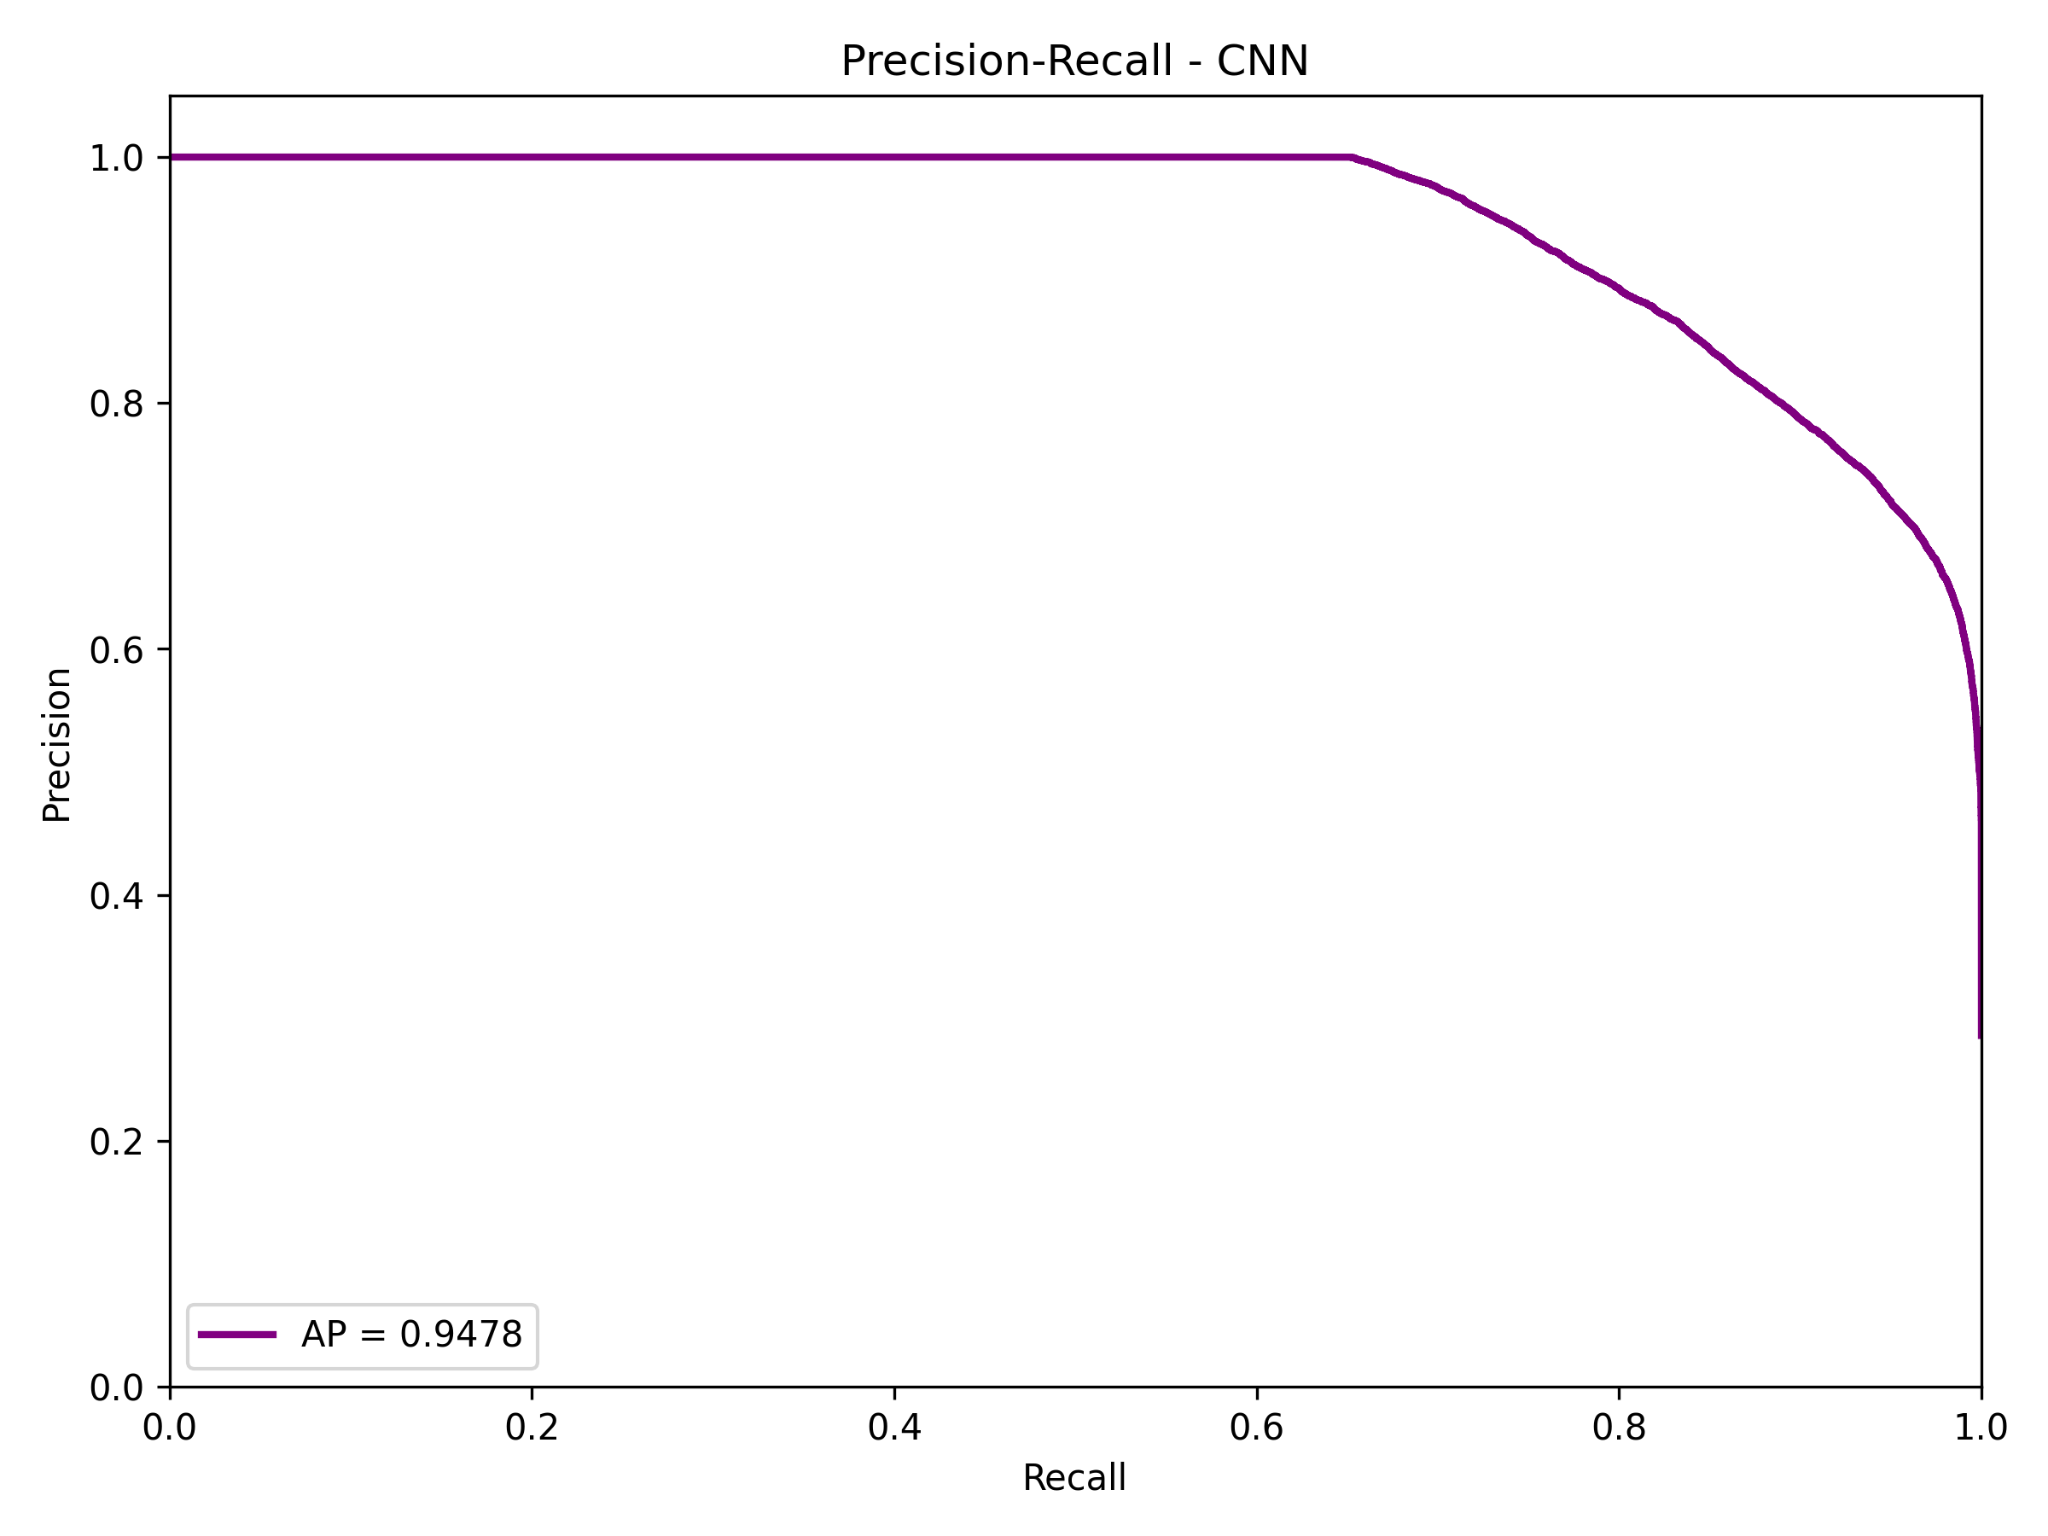
\includegraphics[width=0.4\textwidth]{figuras/pr cnn.png} 
    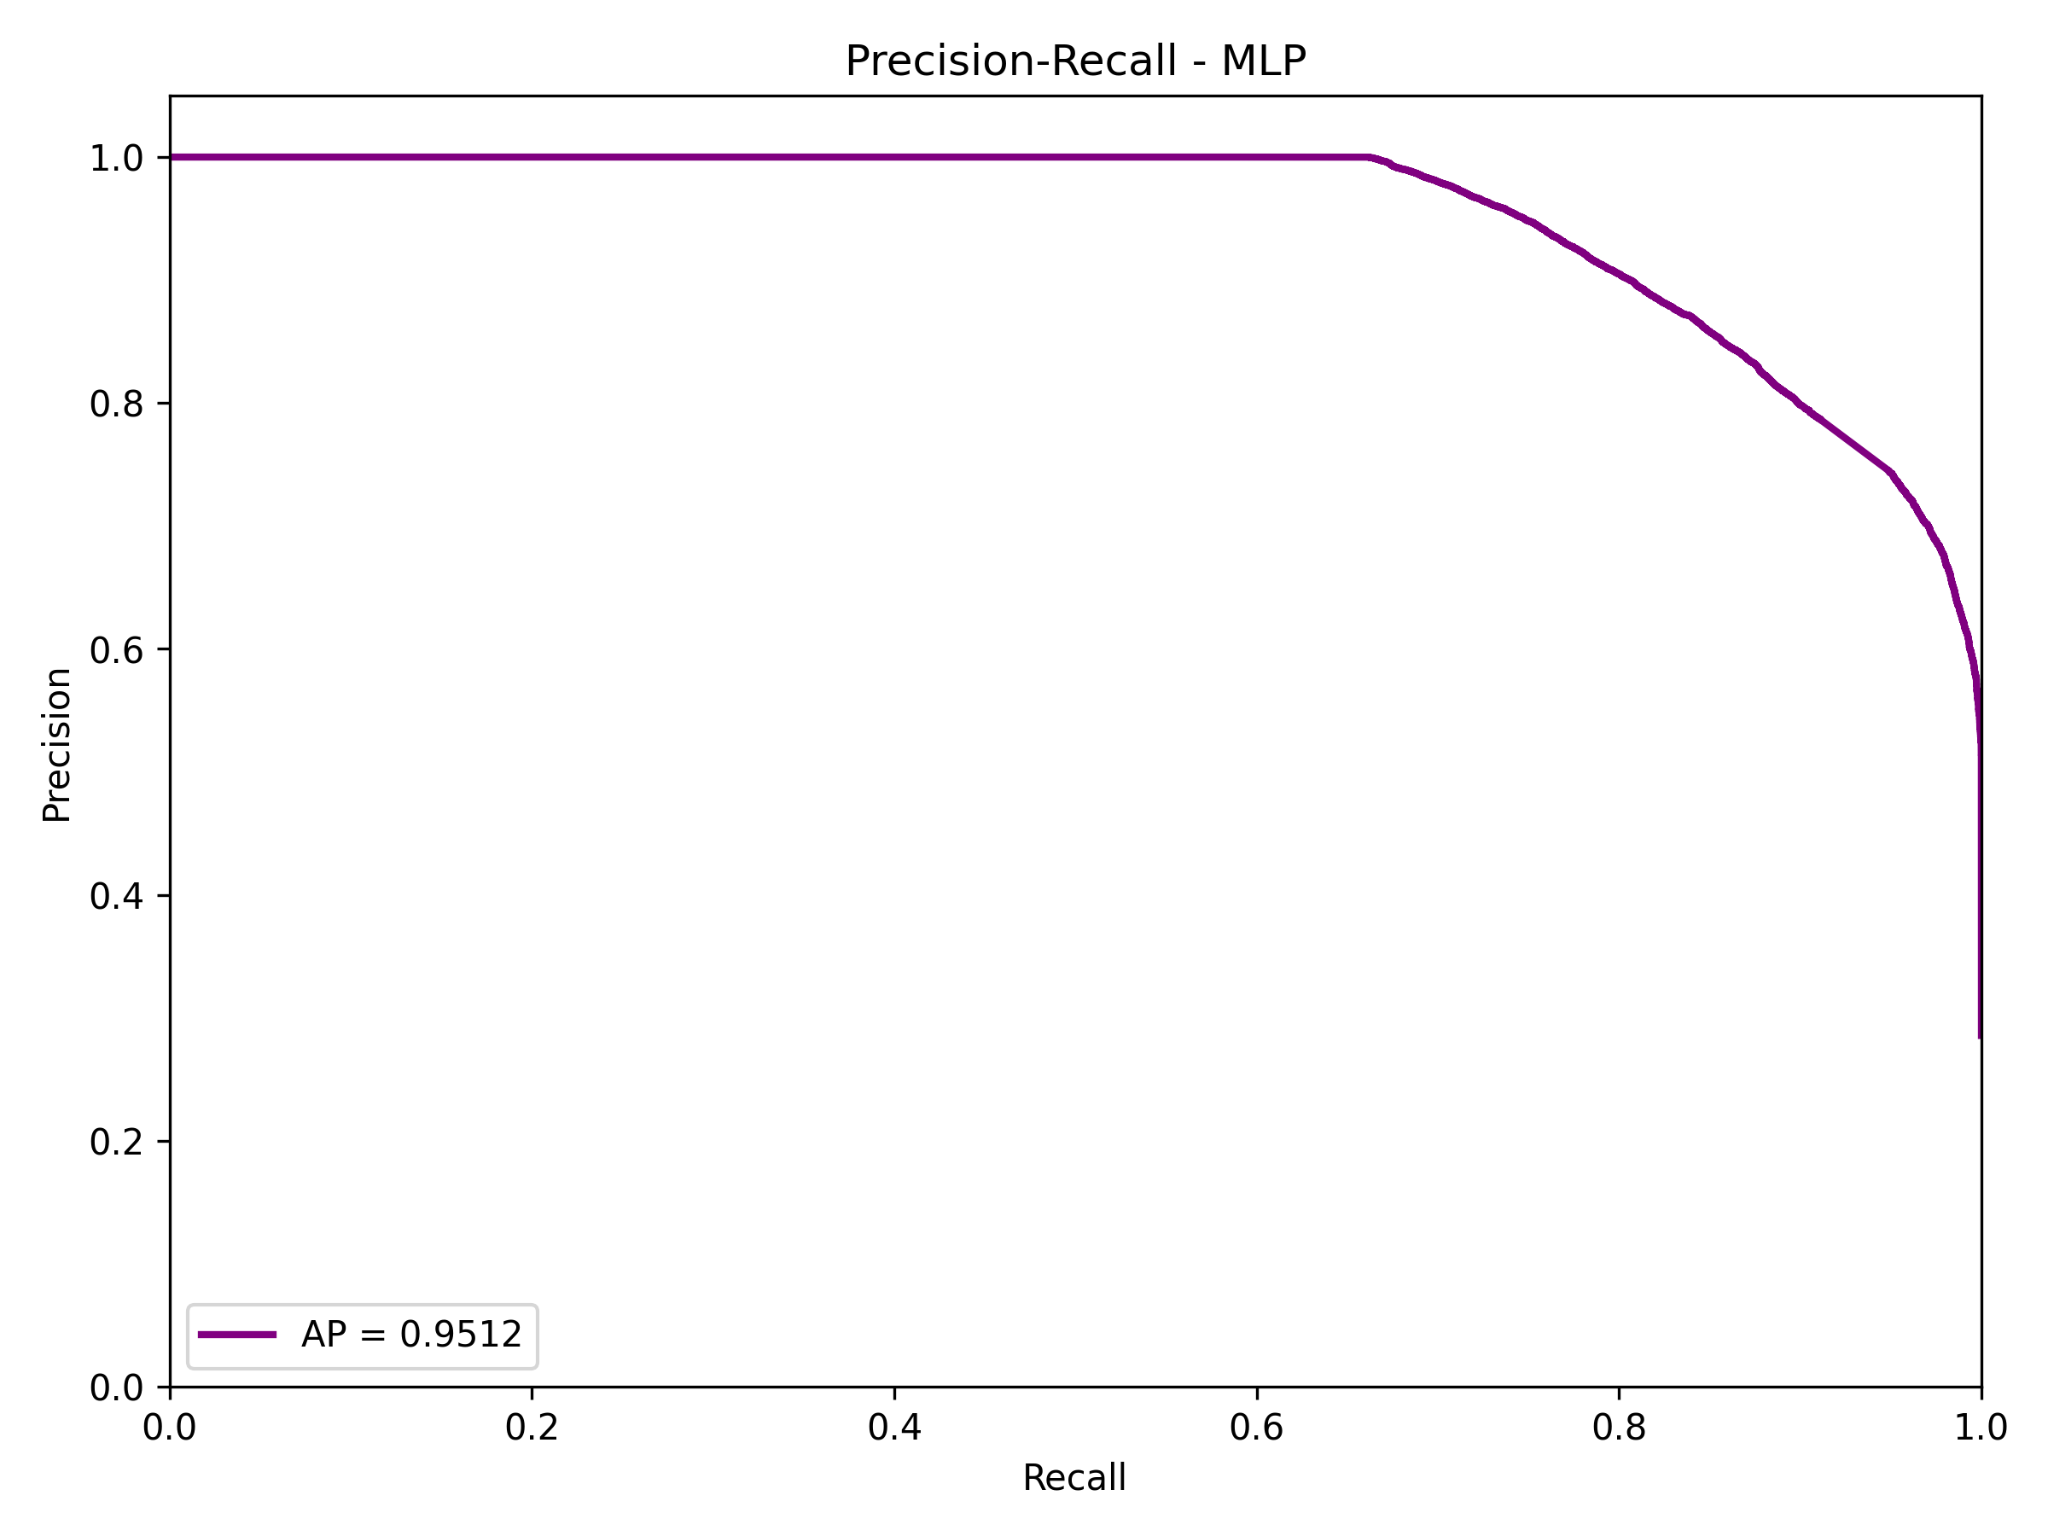
\includegraphics[width=0.4\textwidth]{figuras/pr mlp.png} 
    \par 
     \small Fonte: Elaborado pelo autor
\end{figure}

Na figura 13 podemos ver um exemplo de uma curva precisão-recall ela ilustra a relação inversa entre precisão e recall em diferentes pontos de corte. Um alto valor de área sob a curva indica tanto um recall elevado quanto uma precisão alta. A alta precisão reflete a minimização de falsos positivos nos resultados apresentados, enquanto o alto recall garante que poucos falsos negativos sejam incluídos nos resultados relevantes. Consequentemente, pontuações elevadas em ambos os aspectos sugerem que o classificador oferece resultados exatos e abrange a maioria dos resultados pertinentes. (scikit- learn , 2025)

Esta métrica foi crucial na seleção do modelo final, visto que a minimização de Falsos Negativos era de suma importância para o problema em questão. 

\section{Resultados preliminares e Discussão}
Discutiremos, na sequência, os resultados das explicações geradas pelos métodos aplicados no capítulo anterior.

\subsection{Desempenho}
Trials: Escolhendo o melhor modelo
Aqui vamos mostrar os resultados obtidos 
As Tabelas 2 e 3 exibem, respectivamente, o desempenho dos ensaios para os modelos MLP e CNN. No caso do modelo MLP, optou-se pelo ensaio 19, que apresentou um recall de 80,82\% e precisão de 71,03\%. Para o modelo CNN, o ensaio 19 também foi selecionado devido à sua precisão de 86,93\%, que, apesar de um recall ligeiramente inferior ao do MLP, alinha-se com a estratégia de priorizar o recall. 

% Tabela 2
\begin{table}[H]
    \centering
    \caption{Resultados Trials MPL}
    \label{tab:trials_mlp}
    \begin{tabular}{@{}llllll@{}}
        \toprule
        \textbf{trial\_id} & \textbf{precision} & \textbf{accuracy} & \textbf{recall} & \textbf{loss} & \textbf{auc} \\
        \midrule
        19 & 71.03\% & 95.53\% & 80.82\% & 12.48\% & 88.23\% \\
        7 & 60.62\% & 91.69\% & 84.71\% & 17.64\% & 86.91\% \\
        11 & 61.55\% & 94.19\% & 84.71\% & 13.02\% & 88.23\% \\
        14 & 64.57\% & 94.20\% & 83.76\% & 14.36\% & 88.07\% \\
        17 & 61.97\% & 93.93\% & 83.29\% & 14.48\% & 87.83\% \\
        10 & 69.99\% & 95.43\% & 80.94\% & 11.94\% & 88.04\% \\
        3 & 70.87\% & 95.54\% & 80.71\% & 13.04\% & 88.20\% \\
        12 & 64.00\% & 94.49\% & 80.47\% & 13.30\% & 85.85\% \\
        4 & 60.82\% & 93.90\% & 79.53\% & 21.38\% & 81.85\% \\
        16 & 75.75\% & 95.96\% & 78.71\% & 12.15\% & 88.11\% \\
        6 & 75.17\% & 95.96\% & 78.35\% & 14.53\% & 88.00\% \\
        15 & 76.53\% & 95.11\% & 78.12\% & 13.91\% & 87.93\% \\
        0 & 70.89\% & 95.36\% & 77.29\% & 13.64\% & 86.79\% \\
        2 & 74.95\% & 95.83\% & 77.18\% & 11.28\% & 87.82\% \\
        18 & 80.67\% & 96.25\% & 75.65\% & 13.35\% & 87.30\% \\
        8 & 79.16\% & 95.98\% & 74.24\% & 15.24\% & 86.73\% \\
        13 & 91.82\% & 97.10\% & 72.35\% & 14.67\% & 88.01\% \\
        5 & 93.95\% & 96.97\% & 69.29\% & 14.04\% & 87.36\% \\
        9 & 99.08\% & 96.73\% & 62.12\% & 25.46\% & 85.78\% \\
        1 & 69.14\% & 95.13\% & 77.18\% & 26.49\% & 85.68\% \\
        \bottomrule
    \end{tabular}
\end{table}

% Tabela 3
\begin{table}[H]
    \centering
    \caption{Resultados Trials CNN}
    \label{tab:trials_cnn}
    \begin{tabular}{@{}llllll@{}}
        \toprule
        \textbf{trial\_id} & \textbf{precision} & \textbf{accuracy} & \textbf{auc} & \textbf{recall} & \textbf{loss} \\
        \midrule
        19 & 86.93\% & 96.83\% & 97.48\% & 74.24\% & 13.28\% \\
        8 & 56.30\% & 93.08\% & 96.63\% & 83.18\% & 16.45\% \\
        9 & 63.16\% & 94.41\% & 97.54\% & 82.35\% & 23.15\% \\
        14 & 66.52\% & 94.91\% & 97.50\% & 80.82\% & 14.10\% \\
        1 & 65.17\% & 94.58\% & 97.12\% & 79.65\% & 51.37\% \\
        18 & 68.08\% & 95.01\% & 97.38\% & 78.00\% & 13.56\% \\
        15 & 66.77\% & 94.82\% & 97.00\% & 77.76\% & 27.38\% \\
        10 & 70.53\% & 95.25\% & 97.06\% & 76.12\% & 28.55\% \\
        2 & 75.47\% & 95.77\% & 97.30\% & 74.47\% & 13.59\% \\
        16 & 71.46\% & 95.28\% & 96.84\% & 74.12\% & 22.60\% \\
        3 & 89.50\% & 96.92\% & 97.64\% & 72.35\% & 12.86\% \\
        0 & 83.10\% & 96.35\% & 97.40\% & 71.65\% & 13.26\% \\
        5 & 85.17\% & 96.53\% & 97.54\% & 71.65\% & 12.84\% \\
        6 & 90.11\% & 96.76\% & 97.14\% & 70.12\% & 13.75\% \\
        17 & 88.71\% & 96.66\% & 97.33\% & 69.65\% & 12.63\% \\
        4 & 80.34\% & 95.86\% & 96.97\% & 69.18\% & 15.24\% \\
        12 & 79.76\% & 95.81\% & 96.60\% & 68.00\% & 28.63\% \\
        7 & 89.57\% & 96.40\% & 97.16\% & 65.18\% & 15.55\% \\
        13 & 87.31\% & 95.64\% & 96.23\% & 57.53\% & 15.57\% \\
        \bottomrule
    \end{tabular}
\end{table}

Consequentemente, os modelos escolhidos para as análises comparativas futuras, que foram apresentados na seção 4.2.1.1 , foram cuidadosamente selecionados com base em critérios rigorosos, incluindo a métrica de recall previamente discutida em parágrafos anteriores. Essa seleção visa garantir a relevância e a robustez dos resultados obtidos. Desse modo, a metodologia adotada para a escolha desses modelos é um pilar fundamental dessa pesquisa. 

\subsection{Treinamento}
Após a fase de ajuste, que determinou as configurações ideais de hiperparâmetros, o retreinamento foi realizado no conjunto de treinamento com validação retida. Durante este processo, aplicou-se regularização e controle de sobreajuste por meio de EarlyStopping, que monitorou a pr\_auc, e Model Checkpoint, que salvou o modelo com melhor desempenho com base no mesmo critério. Adicionalmente, utilizou-se ReduceLROnPlateau para o ajuste adaptativo da taxa de aprendizado. Quando necessário, foram incorporados pesos de classe para corrigir assimetrias nas frequências das classes. Ao final, os modelos "best" e "final" foram salvos para garantir a reprodutibilidade. A avaliação de desempenho foi conduzida em um conjunto de teste separado, reportando métricas padronizadas como precisão, revocação, F1 e AUC-ROC. Este protocolo assegura a reprodutibilidade, rastreabilidade e validade externa, em conformidade com as boas práticas de engenharia e experimentação em aprendizado de máquina. 

Os resultados dos treinamentos, para CNN e MLP respectivamente, estão apresentados nas tabelas 4 e 5. 

% Tabela 4
\begin{table}[H]
    \centering
    \caption{Resultados do treinamento CNN}
    \label{tab:train_cnn}
    \begin{tabular}{@{}lllll@{}}
        \toprule
        \textbf{metric} & \textbf{mean} & \textbf{std} & \textbf{min} & \textbf{max} \\
        \midrule
        loss & 23.91\% & 0.61\% & 23.48\% & 28.48\% \\
        accuracy & 88.96\% & 0.17\% & 87.83\% & 89.16\% \\
        precision & 75.41\% & 0.31\% & 73.49\% & 75.80\% \\
        recall & 91.05\% & 0.21\% & 89.79\% & 91.37\% \\
        auc & 97.04\% & 0.11\% & 96.19\% & 97.11\% \\
        \bottomrule
    \end{tabular}
\end{table}

% Tabela 5
\begin{table}[H]
    \centering
    \caption{Resultados do treinamento MLP}
    \label{tab:train_mlp}
    \begin{tabular}{@{}lllll@{}}
        \toprule
        \textbf{metric} & \textbf{mean} & \textbf{std} & \textbf{min} & \textbf{max} \\
        \midrule
        loss & 21.64\% & 1.85\% & 19.60\% & 29.04\% \\
        accuracy & 89.11\% & 0.57\% & 87.56\% & 89.88\% \\
        precision & 75.37\% & 1.06\% & 73.00\% & 76.84\% \\
        recall & 91.98\% & 0.47\% & 89.62\% & 92.65\% \\
        auc & 97.18\% & 0.32\% & 96.06\% & 97.55\% \\
        \bottomrule
    \end{tabular}
\end{table}

Observa-se que o modelo MLP superou ligeiramente o modelo que utiliza a arquitetura CNN, embora a diferença não seja muito significativa. 
